\documentclass[10pt]{mypackage}

% sans serif font:
%\usepackage{cmbright}
%\usepackage{sfmath}
%\usepackage{bbold} %better blackboard bold

%serif font + different blackboard bold for serif font
\usepackage{newpxtext,eulerpx}
\renewcommand*{\mathbb}[1]{\varmathbb{#1}}
\renewcommand*{\hbar}{\hslash}

\pagestyle{fancy} %better headers
\fancyhf{}
\rhead{Avinash Iyer}
\lhead{Ordinary Differential Equations: Homework 8}

\setcounter{secnumdepth}{0}

\begin{document}
\RaggedRight
\section{Part 1}%
\subsection{2.6, Problem 2}%
\begin{enumerate}[(a)]
  \item Using Mathematica and effective guessing, we land upon an initial condition of $\vec{Y}(0) = \begin{pmatrix}0\\2.13\end{pmatrix}$.
  \item All solutions with initial conditions in this curve will have the same periodic solution.
\end{enumerate}
\subsection{2.6, Problem 3}%
\begin{align*}
  \diff{\vec{Y}_1}{t} &= \diff{}{t} \begin{pmatrix}e^{-t}\sin(3t)\\e^{-t}\cos(3t)\end{pmatrix}\\
                      &= \begin{pmatrix}-e^{-t}\sin(3t) + 3e^{-t}\cos(3t) \\ -e^{-t}\cos(3t) - 3e^{-t}\sin(3t)\end{pmatrix}\\
                      &= \begin{pmatrix}-x+3y\\-3x-y\end{pmatrix}.
\end{align*}
\subsection{2.6, Problem 4}%
Since $\vec{Y}_2(t) = \vec{Y}_1\left(t-1\right)$ and $\vec{Y}_1(t)$  is a solution, so too is $\vec{Y}_2(t)$.
\subsection{2.6, Problem 5}%
Plotting, we see the following.
\begin{center}
  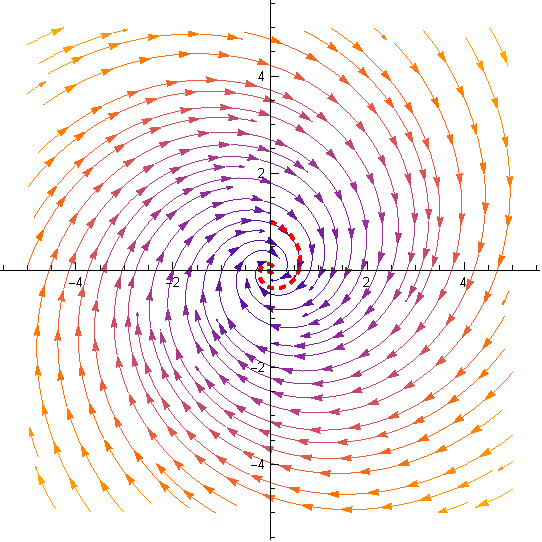
\includegraphics[width=7cm]{images/2_6_5a.pdf} 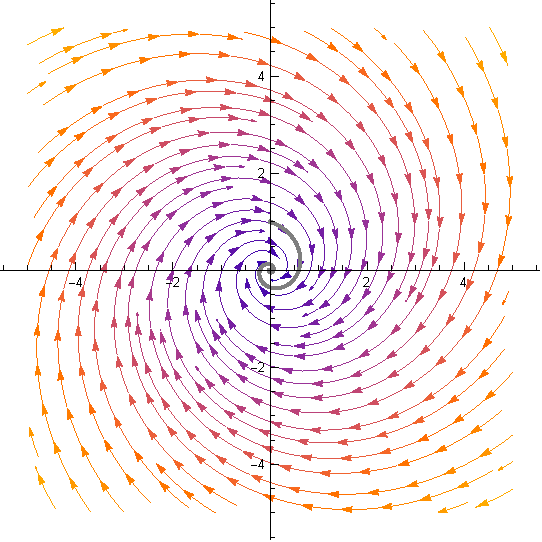
\includegraphics[width=7cm]{images/2_6_5b.pdf}
\end{center}
This does not violate the uniqueness theorem since if $t_0 = 0$ for $\vec{Y}_1$ and $t_0 = 1$ for $\vec{Y}_1$, then the solutions are exactly the same.
\subsection{2.6, Problem 9}%
We must have $\vec{Y}_1$ is a phase shift of $\vec{Y}_2$. Specifically, $\vec{Y}_1(t) = \vec{Y}_2(t-1)$.
\subsection{Chapter 2 Review, Problem 2}%
Solving $\diff{x}{t}$, we must have $y=0$, which yields $\diff{y}{t} = x^2 + 1$. Therefore, there are no equilibrium solutions for this equation.
\subsection{Chapter 2 Review, Problem 3}%
\begin{align*}
  x &= \diff{y}{t}\\
  \diff{x}{t} &= 1
\end{align*}
\subsection{Chapter 2 Review, Problem 7}%
\begin{align*}
  \diff{x}{t} &= -6e^{-6t}\\
              &= 2\left(e^{-6t}\right) - 2\left(4e^{-6t}\right)\\
              &= 2x - 2y^2\\
  \diff{y}{t} &= -6e^{-3t}\\
              &= -3y.
\end{align*}
Thus, this is a solution to the system of differential equations.
\subsection{Chapter 2 Review, Problem 12}%
\begin{align*}
  \vec{Y}\left(0.5\right) &\approx \vec{Y}(0) + 0.5\vec{F}\left(\vec{Y}(0)\right)\\
                          &= \begin{pmatrix}3.5\\2\end{pmatrix}.
\end{align*}
\subsection{Chapter 2 Review, Problem 13}%
\begin{center}
  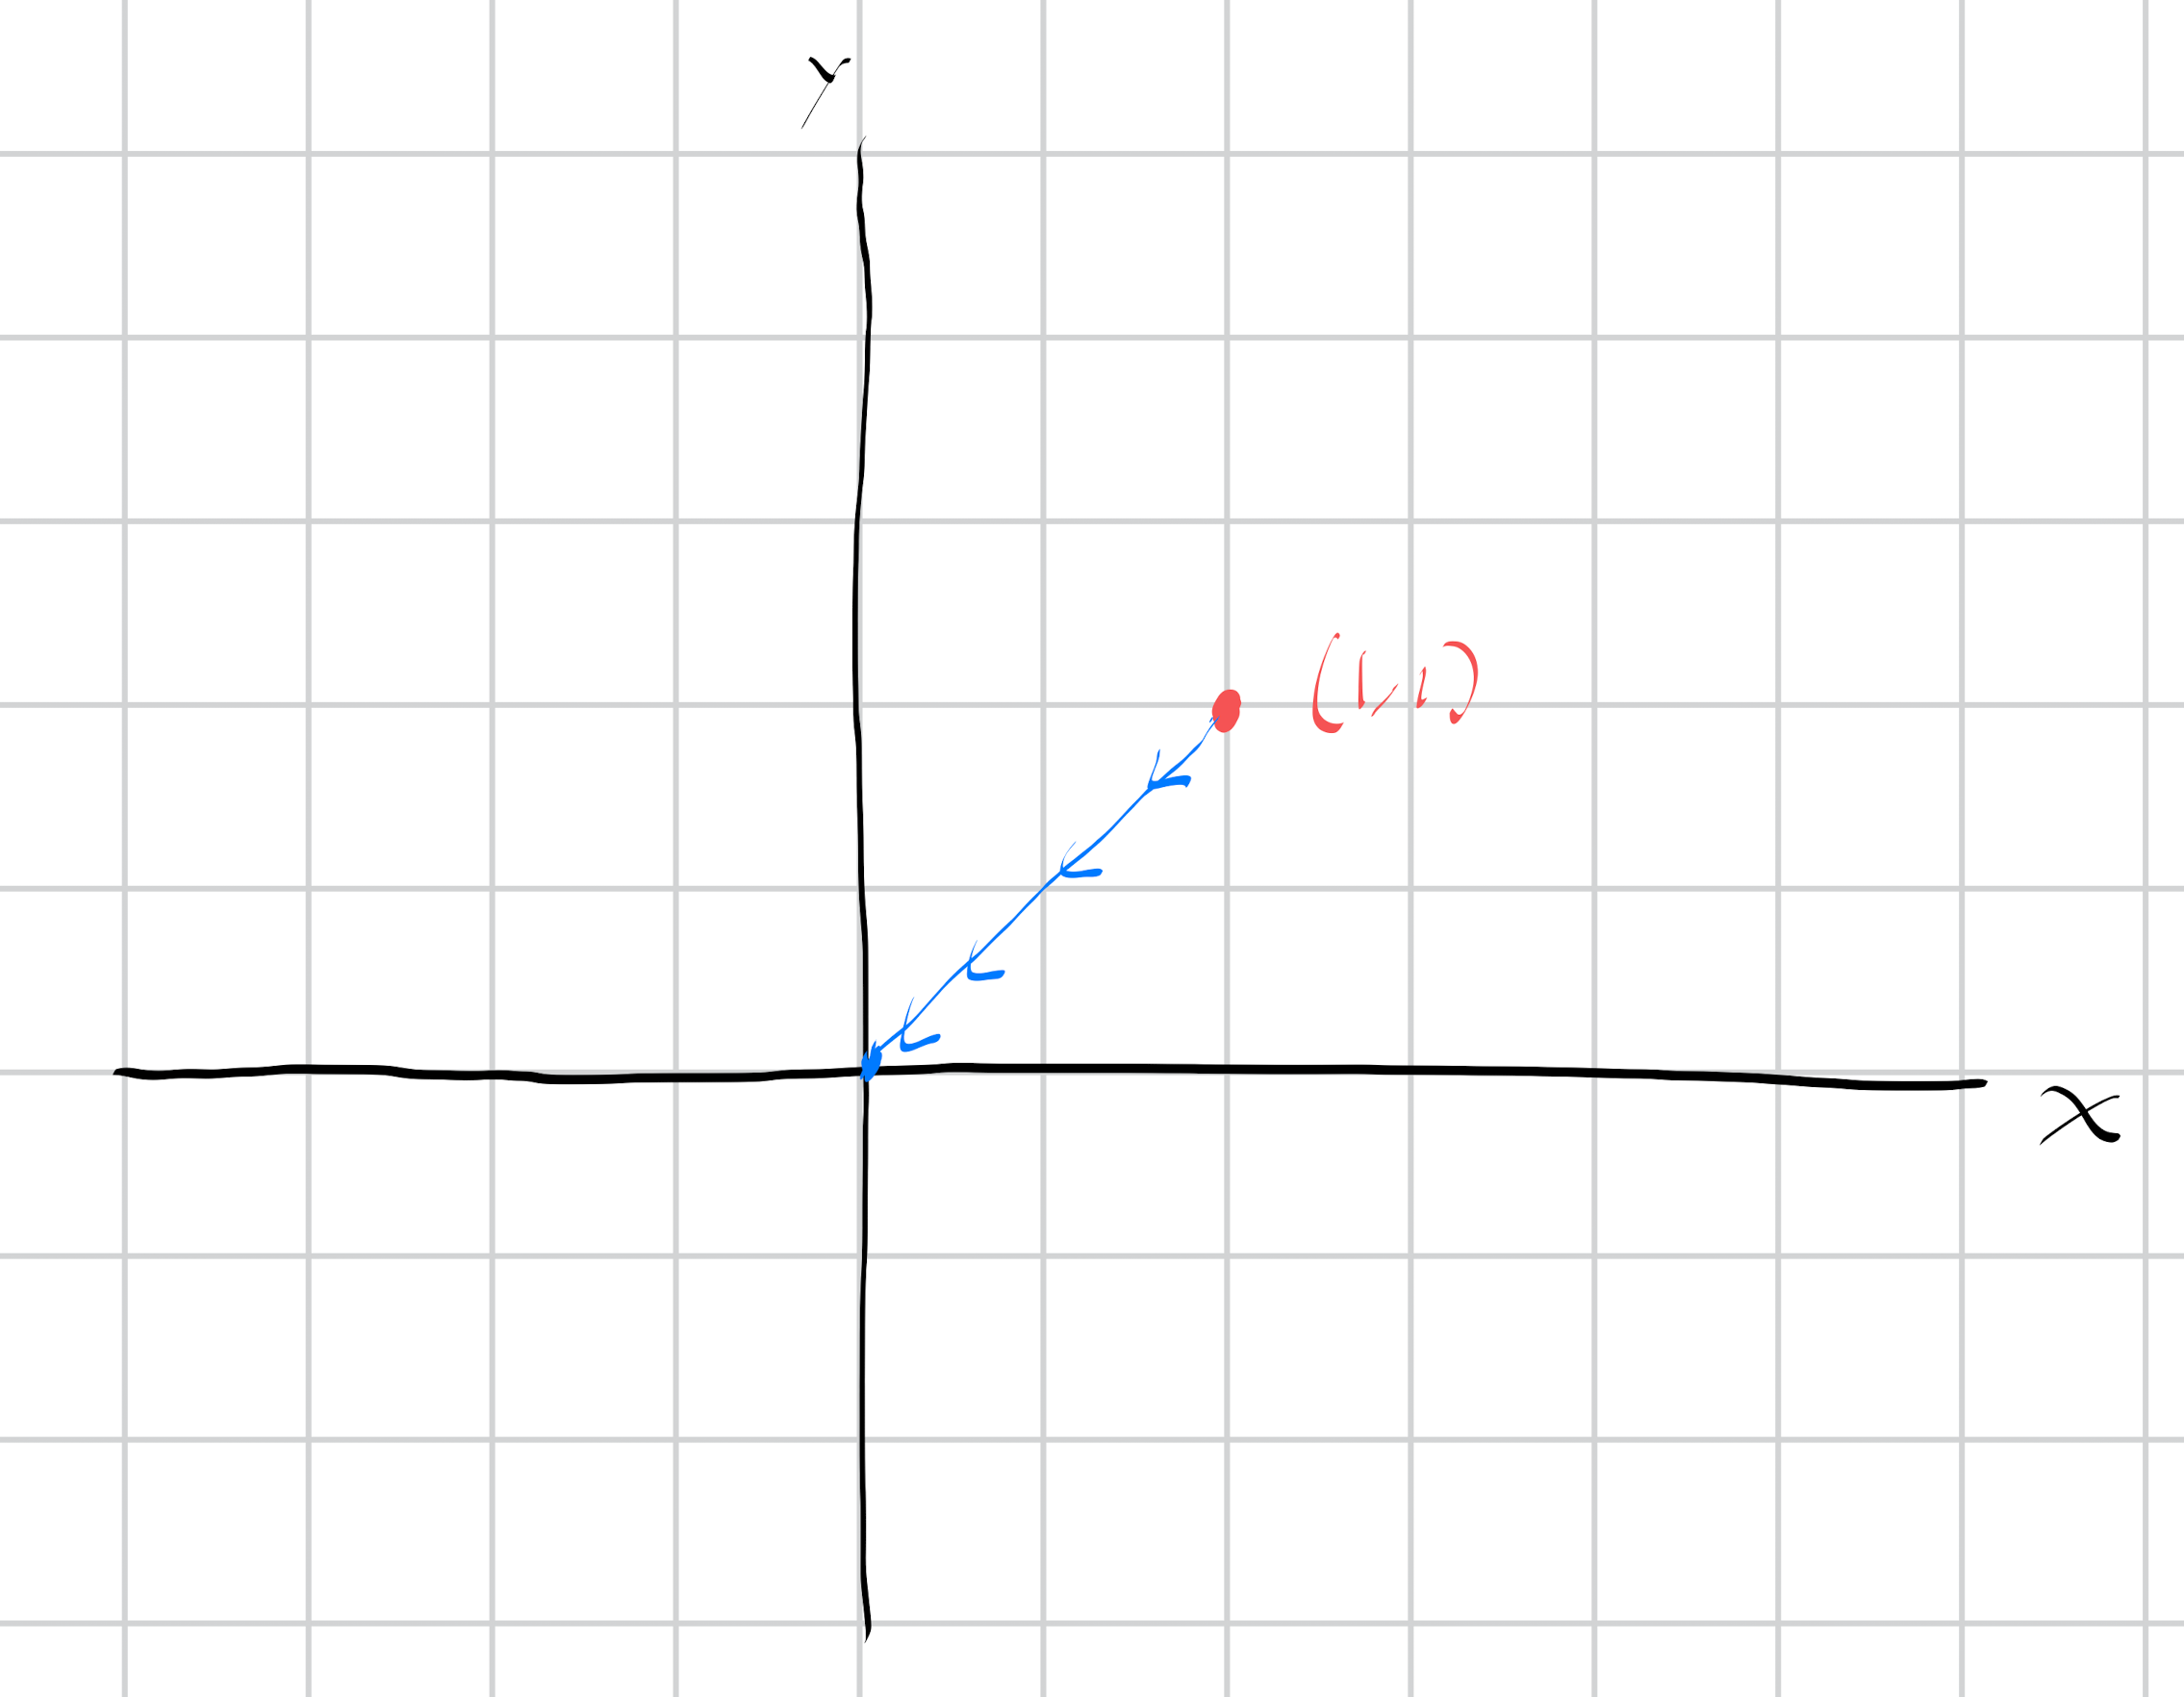
\includegraphics[width=7cm]{images/2_review_13.png}
\end{center}
\subsection{Chapter 2 Review, Problem 15}%
This is true, as we have shown in the solution to Problem 7.
\subsection{Chapter 2 Review, Problem 16}%
This is true, as $y = 0$ means $\diff{y}{t} = 0 = -y$, and for $x(t) = 2$, $\diff{x}{t} = 0$, meaning this is an equilibrium solution to the differential equation.
\subsection{Chapter 2 Review, Problem 20}%
This is true, as phase shifting any solution to a system of differential equations yields another solution to a system of differential equations.
\subsection{Chapter 2 Review, Problem 30}%
The phase portrait of the completely decoupled system has all its solution curves as lines.
\subsection{3.1, Problem 6}%
\begin{align*}
  \diff{\vec{Y}}{t} &= \begin{pmatrix}0 & 3 \\ -0.3 & 3\pi\end{pmatrix} \begin{pmatrix}x(t)\\y(t)\end{pmatrix}.
\end{align*}
\subsection{3.1, Problem 7}%
\begin{align*}
  \diff{\vec{Y}}{t} &= \begin{pmatrix}3 & -2 & 7 \\ -2 & 0 & 6 \\ 0 & 7.3 & 2\end{pmatrix} \begin{pmatrix}p(t)\\q(t)\\r(t)\end{pmatrix}
\end{align*}
\subsection{3.1, Problem 8}%
\begin{align*}
  \diff{x}{t} &= -3x + 2\pi y\\
  \diff{y}{t} &= 4x-y.
\end{align*}
\section{Part 2}%
\subsection{3.1, Problem 10}%
\begin{center}
  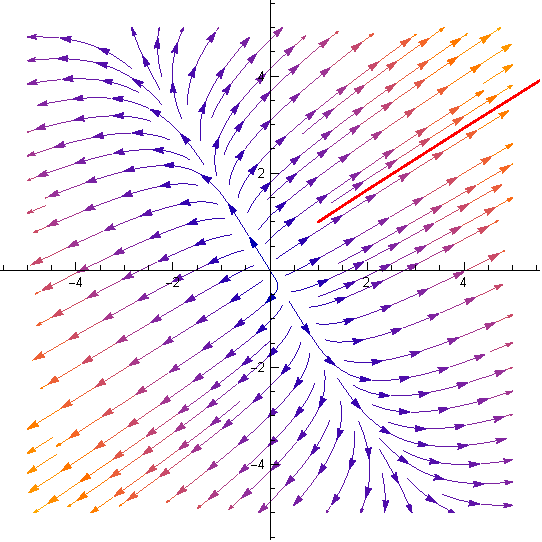
\includegraphics[width=7cm]{images/3_1_10_a.pdf} 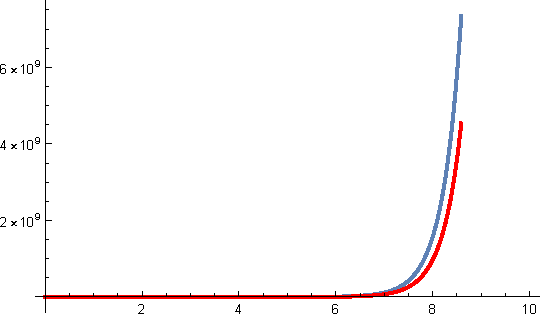
\includegraphics[width=7cm]{images/3_1_10_b.pdf}
\end{center}
\subsection{3.1, Problem 13}%
\begin{center}
  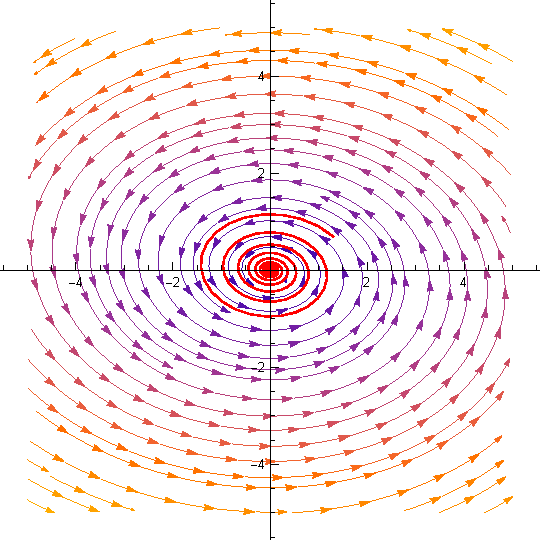
\includegraphics[width=7cm]{images/3_1_13_a.pdf} 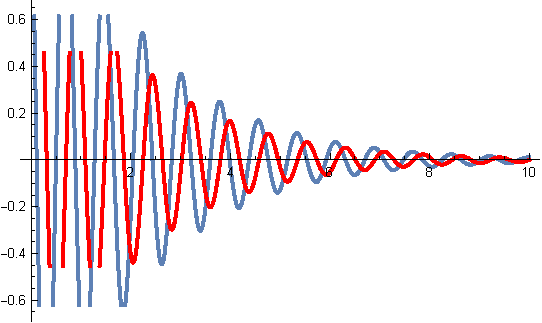
\includegraphics[width=7cm]{images/3_1_13_b.pdf}
\end{center}
\subsection{3.1, Problem 18}%
\begin{enumerate}[(a)]
  \item Converting 
    \begin{align*}
      \diff{y}{t} &= v\\
      \diff{v}{t} &= 0,
    \end{align*}
    we have
    \begin{align*}
      v(t) &= c
    \end{align*}
    for some $c$.
  \item This means $y(t) = ct + k$ for $k\in \R$.
  \item 
\end{enumerate}
\subsection{3.1, Problem 31}%
\begin{enumerate}[(a)]
  \item Since
    \begin{align*}
      3 \begin{pmatrix}x_1\\y_1\end{pmatrix} + 0 \begin{pmatrix}x_2\\y_2\end{pmatrix} &= \begin{pmatrix}0\\0\end{pmatrix},
    \end{align*}
    these vectors are not linearly independent.
  \item 
    \begin{align*}
      - \lambda \begin{pmatrix}x_1\\y_1\end{pmatrix} + \lambda \begin{pmatrix}x_2\\y_2\end{pmatrix} = \begin{pmatrix}0\\0\end{pmatrix},
    \end{align*}
    so they are not linearly independent.
  \item If $x_1 \neq 0$, then $y_2 = \frac{x_2y_1}{x_1}$, meaning $y_2 = \lambda y_1$ and $x_2 = \lambda x_1$, so we use (b). Similarly, if $x_2\neq 0$, we take $-\left(x_1y_2 - x_2y_1\right) = x_2y_1 - x_1y_2 = 0$ and use (b) again. Finally, if $x_1 = 0$, then we must have $y_1$ or $x_2 = 0$, both of which yield linear dependence.
\end{enumerate}
\subsection{3.1, Problem 32}%
Let
\begin{align*}
  x_1y_2 - x_2y_1 &\neq 0
\end{align*}
Suppose toward contradiction that $ \begin{pmatrix}x_1\\y_1\end{pmatrix} $ and $ \begin{pmatrix}x_2\\y_2\end{pmatrix} $ are not linearly independent. Then, there is $\lambda$ such that $ \begin{pmatrix}x_1 \\ y_1\end{pmatrix} = \lambda \begin{pmatrix}x_2\\y_2\end{pmatrix} $, meaning we have
\begin{align*}
  x_1y_2 - x_2y_1 &= \lambda x_2y_2 - x_2\lambda y_2
                  &= 0.
\end{align*}
Thus, we must have $ \begin{pmatrix}x_1\\y_1\end{pmatrix} $ and $ \begin{pmatrix}x_2\\y_2\end{pmatrix} $ not linearly independent.
\subsection{3.1, Problem 35}%
\begin{enumerate}[(a)]
  \item 
    \begin{align*}
      \diff{W}{t} &= x_1'(t)y_2(t) + x_1(t)y_2'(t) - \left(x_2'(t)y_1(t) + x_2(t)y_1'(t)\right).
    \end{align*}
  \item 
    \begin{align*}
      \diff{W}{t} &= x_1'(t)y_2(t) + x_1(t)y_2'(t) - \left(x_2'(t)y_1(t) + x_2(t)y_1'(t)\right)\\
                  &= \left(ax_1(t) + by_1(t)\right)y_2(t) + x_1(t)\left(cx_2(t) + dy_2(t)\right) - \left(\left(ax_2(t) + by_2(t)\right)y_1(t) + x_2(t)\left(ax_1(t) + by_1(t)\right)\right)\\
                  &= \left(a+d\right)\left(x_1(t)y_2(t) - x_2(t)y_1(t)\right)\\
                  &= \left(a+d\right)W(t).
    \end{align*}
  \item 
    \begin{align*}
      \diff{W}{t} &= \left(a+d\right)W(t)\\
      W(t)  &= e^{\left(a+d\right)t}.
    \end{align*}
  \item 
    \begin{align*}
      W(0) &= x_1(0)y_2(0) - x_2(0)y_1(0)\\
           &= \det \begin{pmatrix}x_1(0) & x_2(0) \\ y_1(0) & y_2(0)\end{pmatrix}\\
           &\neq 0,
    \end{align*}
    meaning
    \begin{align*}
      \diff{W}{t} &= \left(a+d\right)W(t)
    \end{align*}
    has a nondegenerate initial condition. Thus, we have
    \begin{align*}
      W(t) &= e^{\left(a+d\right)t},
    \end{align*}
    which is never zero, meaning $\vec{Y}_1(t)$ and $\vec{Y}_2(t)$ are always linearly independent.
\end{enumerate}
\subsection{3.2, Problem 8}%
\subsection{3.2, Problem 9}%
\subsection{3.2, Problem 12}%
\subsection{3.2, Problem 16}%
\subsection{3.2, Problem 17}%
\subsection{3.2, Problem 18}%


\end{document}
